\documentclass[compress]{beamer}
\usepackage{ifthen,verbatim,hyperref,ulem}

\newcommand{\isnote}{}
\xdefinecolor{lightyellow}{rgb}{1.,1.,0.25}
\xdefinecolor{darkblue}{rgb}{0.1,0.1,0.7}

%% Uncomment this to get annotations
\def\notes{\addtocounter{page}{-1}
           \renewcommand{\isnote}{*}
	   \beamertemplateshadingbackground{white}{white}
           \begin{frame}
           \frametitle{Extra notes for page \insertpagenumber}
           \itemize}
\def\endnotes{\enditemize
	      \end{frame}
              \beamertemplateshadingbackground{white}{white}
              \renewcommand{\isnote}{}}

%% Uncomment this to not get annotations
%% \def\notes{\comment}
%% \def\endnotes{\endcomment}

\setbeamertemplate{navigation symbols}{}
\setbeamertemplate{headline}{\mbox{ } \hfill
\begin{minipage}{5.5 cm}
\vspace{-0.75 cm} \small
\end{minipage} \hfill
\begin{minipage}{4.5 cm}
\vspace{-0.75 cm} \small
\begin{flushright}
\ifthenelse{\equal{\insertpagenumber}{1}}{}{Jim Pivarski \hspace{0.2 cm} \insertpagenumber\isnote/14}
\end{flushright}
\end{minipage}\mbox{\hspace{0.2 cm}}\includegraphics[height=1 cm]{../cmslogo} \hspace{0.1 cm} \includegraphics[height=1 cm]{../tamulogo} \hspace{0.01 cm} \vspace{-1.05 cm}}

\begin{document}
\begin{frame}
\vfill
\begin{center}
\textcolor{darkblue}{\Large Magnetic Field from a Muon Alignment Perspective \\ \vspace{0.5 cm} \LARGE Errata}

\vfill
\begin{columns}
\column{0.3\linewidth}
\begin{center}
\large
\textcolor{darkblue}{Jim Pivarski}

\vspace{0.2 cm}
Alexei Safonov
\end{center}
\end{columns}

\begin{columns}
\column{0.3\linewidth}
\begin{center}
\scriptsize
{\it Texas A\&M University}
\end{center}
\end{columns}

\vfill
 2 February, 2009

\end{center}
\end{frame}

%% \begin{notes}
%% \item This is the annotated version of my talk.
%% \item If you want the version that I am presenting, download the one
%% labeled ``slides'' on Indico (or just ignore these yellow pages).
%% \item The annotated version is provided for extra detail and a written
%% record of comments that I intend to make orally.
%% \item Yellow notes refer to the content on the {\it previous} page.
%% \item All other slides are identical for the two versions.
%% \end{notes}

\small

\setcounter{page}{8}

\begin{frame}
\frametitle{Residuals differences plots}

\vspace{0.3 cm}
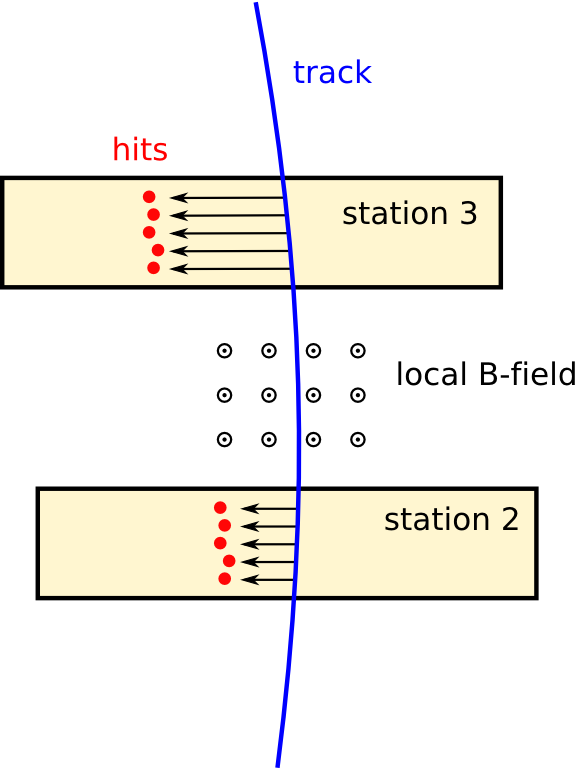
\includegraphics[height=4.4 cm]{residuals_difference.png} 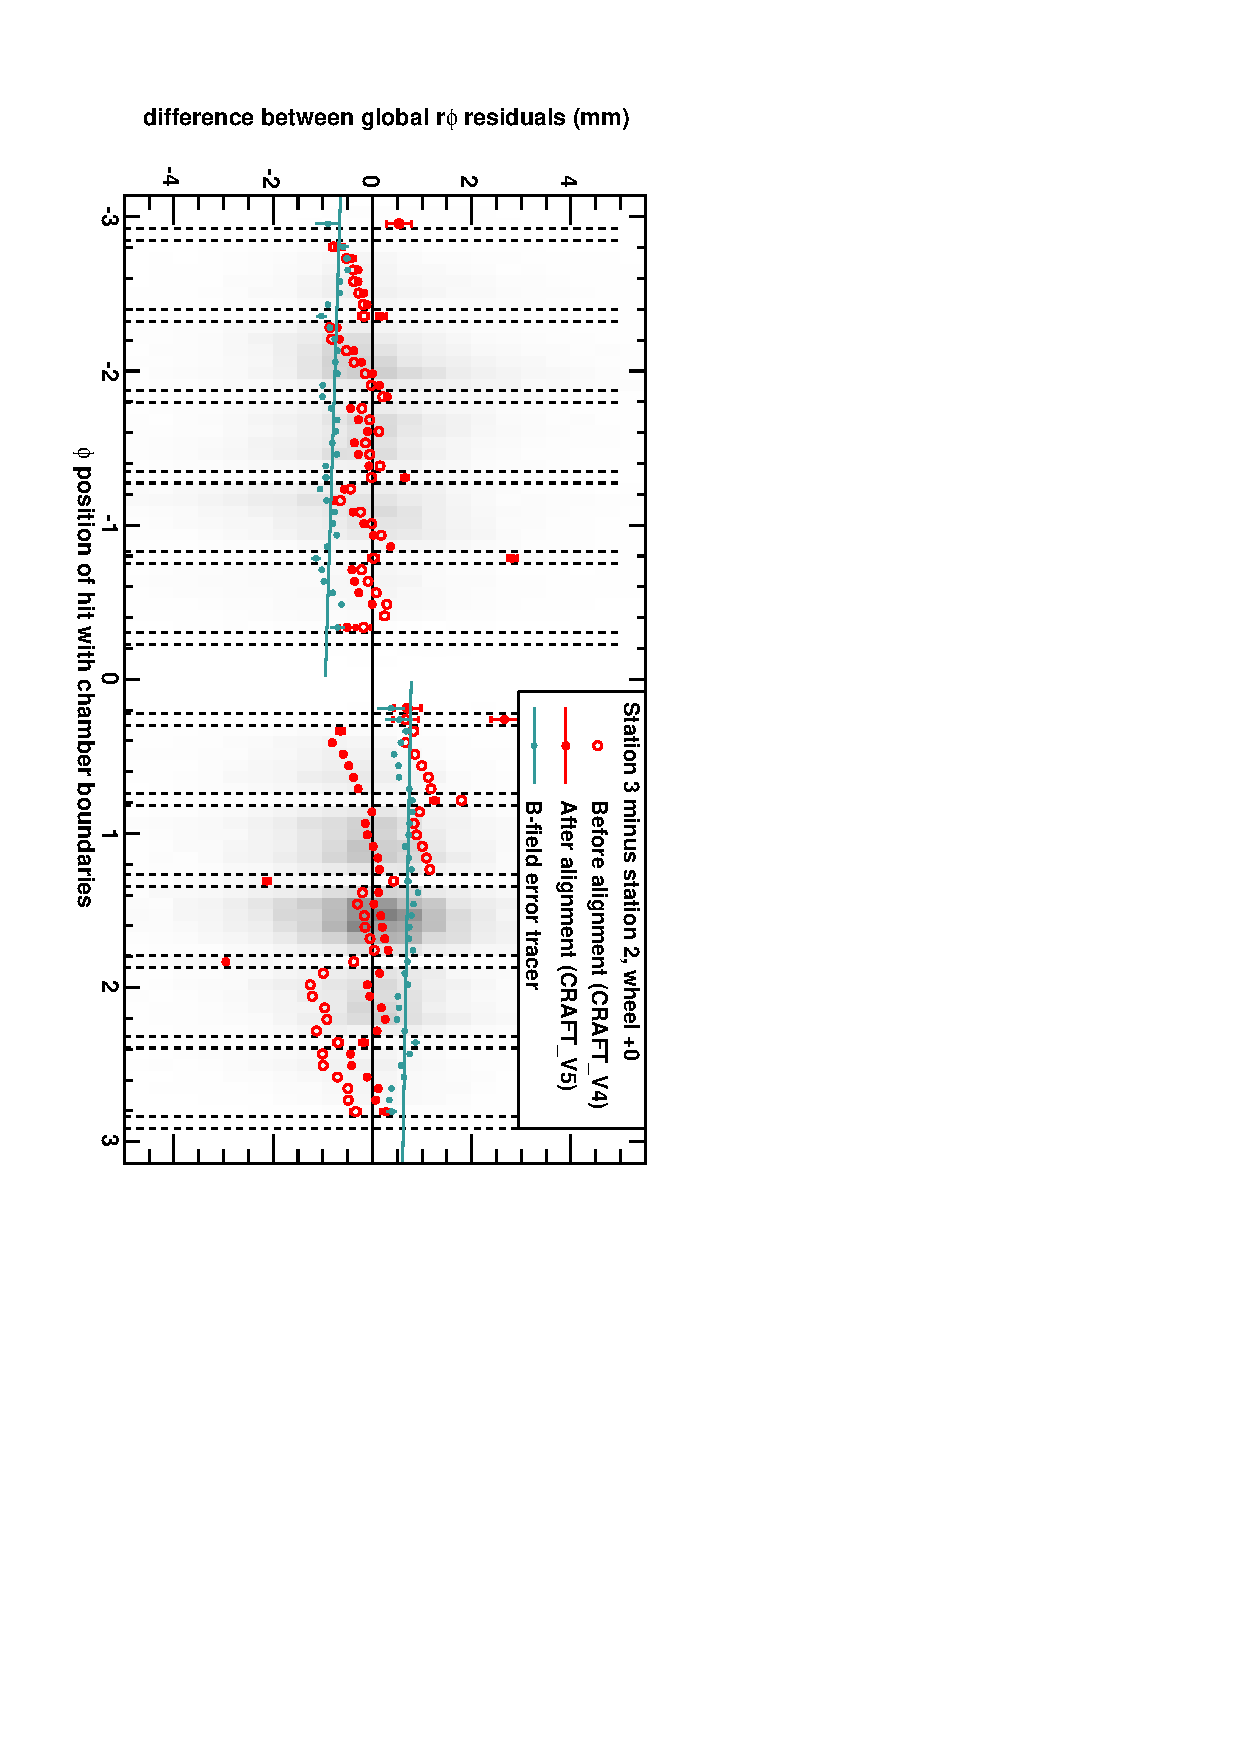
\includegraphics[width=4.5 cm, angle=90]{bfieldtalk_example4.pdf}

\vspace{-0.3 cm}
\begin{itemize}
\item \sout{Also sensitive to local $\vec{B}$-field error, rather than integral over path}
\item Not exactly: see diagram on next page
\end{itemize}
\end{frame}

\begin{notes}
\item Difference between propagated track and real muon grow
  quadratically in regions where the $B_z$ is mismodelled

\item But they also grow linearly in between

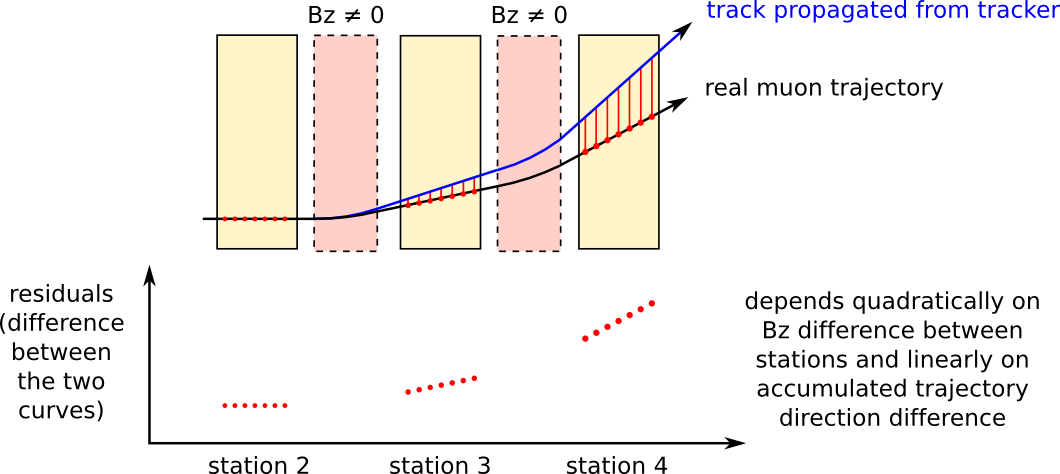
\includegraphics[width=\linewidth]{paths.png}

\item Residuals differences method only sets the ``initial
  displacement'' to zero, it does not set the ``initial velocity'' to
  zero, as would be needed to make the station~3 residuals independent
  of $\vec{B}$-field errors already accumulated in station~2
\end{notes}

\setcounter{page}{9}

\begin{frame}
\frametitle{Calculating $B_z$ error in Tesla}

\vspace{0.3 cm}
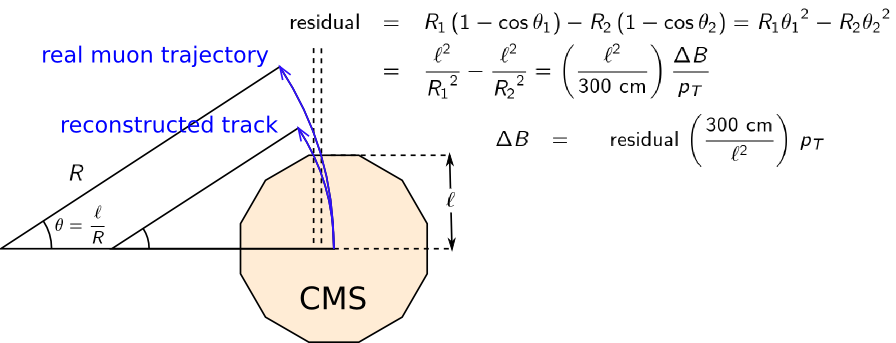
\includegraphics[width=\linewidth]{geometry.png}

\begin{columns}
\column{0.5\linewidth}
\mbox{ }

\scriptsize P.\ Martinez: $r\phi$ residual vs.\ $q/p_T$ \mbox{by station\hspace{-1 cm}}

\vspace{0.05 cm}
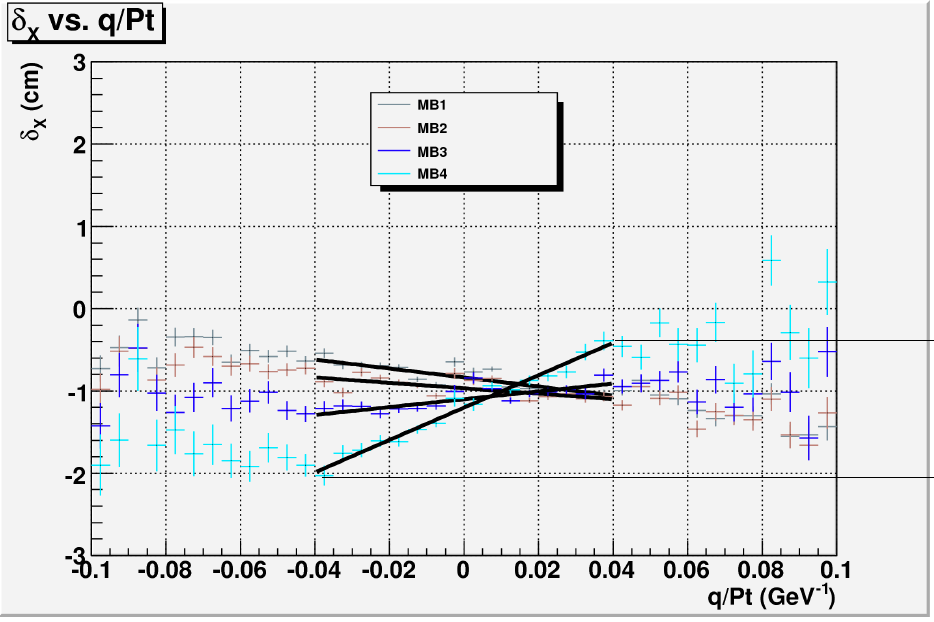
\includegraphics[width=\linewidth]{pmartinez.png}

\column{0.5\linewidth}

\vspace{-3.2 cm}
\begin{itemize}
\item only problem here: $(1 - \cos\theta) \approx \theta^2/2$, not $\theta^2$
\item this multiplies all $\Delta B$ calculations by a factor of two ({\it worse} discrepancy)
\end{itemize}

\vspace{-1.5 cm}
\mbox{ }
\end{columns}
\end{frame}

\setcounter{page}{11}

\begin{frame}
\frametitle{$B_z$ error between stations \only<1>{1\&2}\only<2>{2\&3}\only<3>{3\&4}}

\begin{itemize}
\item As stated on slide 9, these $\Delta B$ values need to be {\it doubled}
\item But they are also susceptible to accumulated track-direction
  errors, so the $\Delta B$ are increasingly exaggerated with station
  number
\item I'm looking into ways of correcting for this
\end{itemize}

\vfill
\only<1>{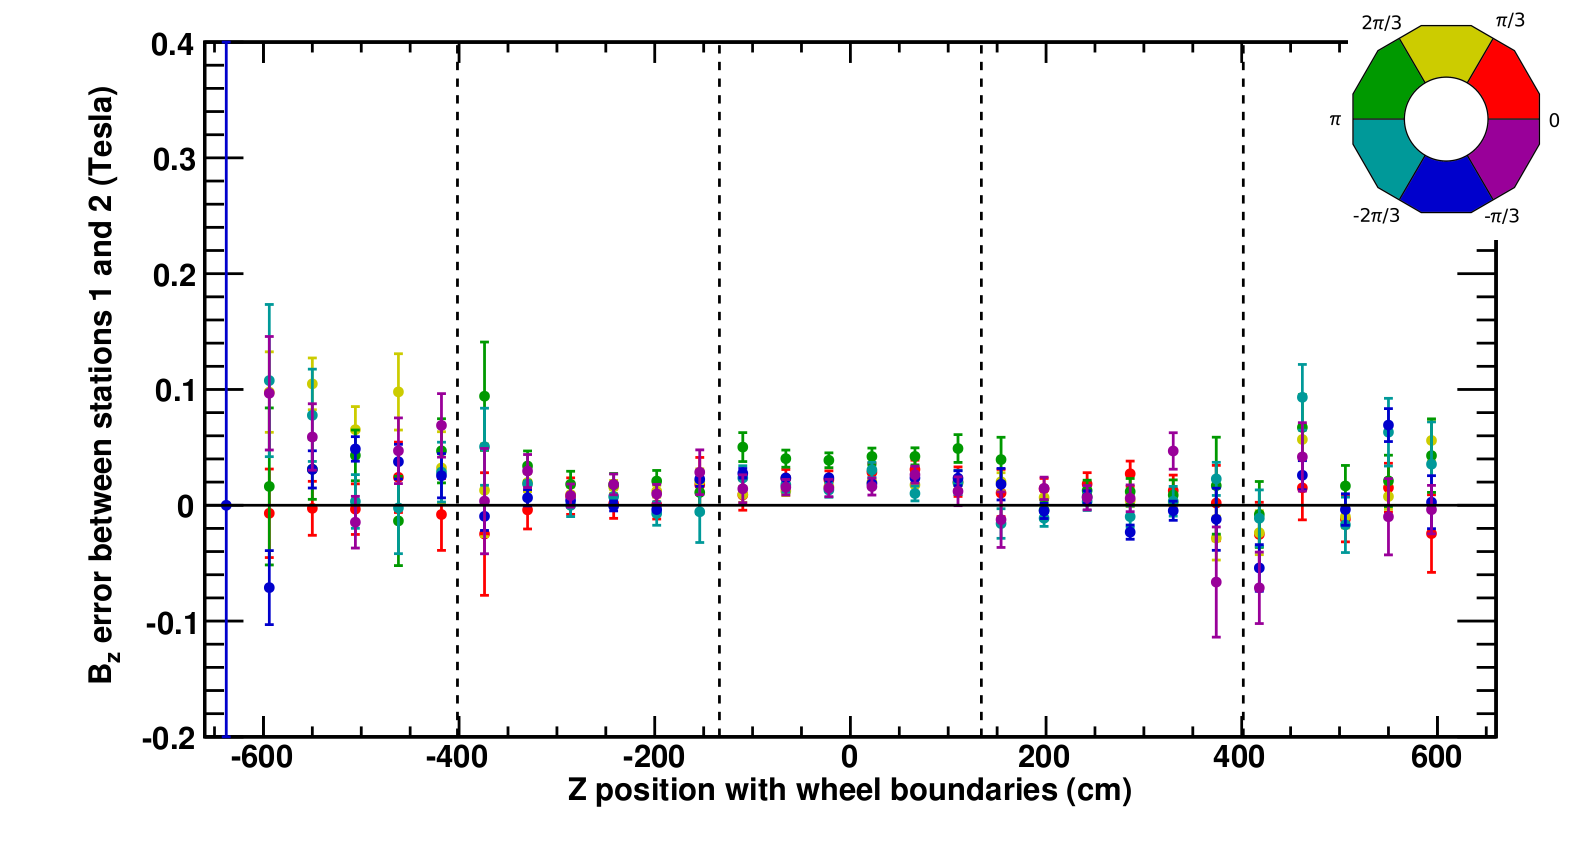
\includegraphics[width=0.95\linewidth]{berror12.png}}
\only<2>{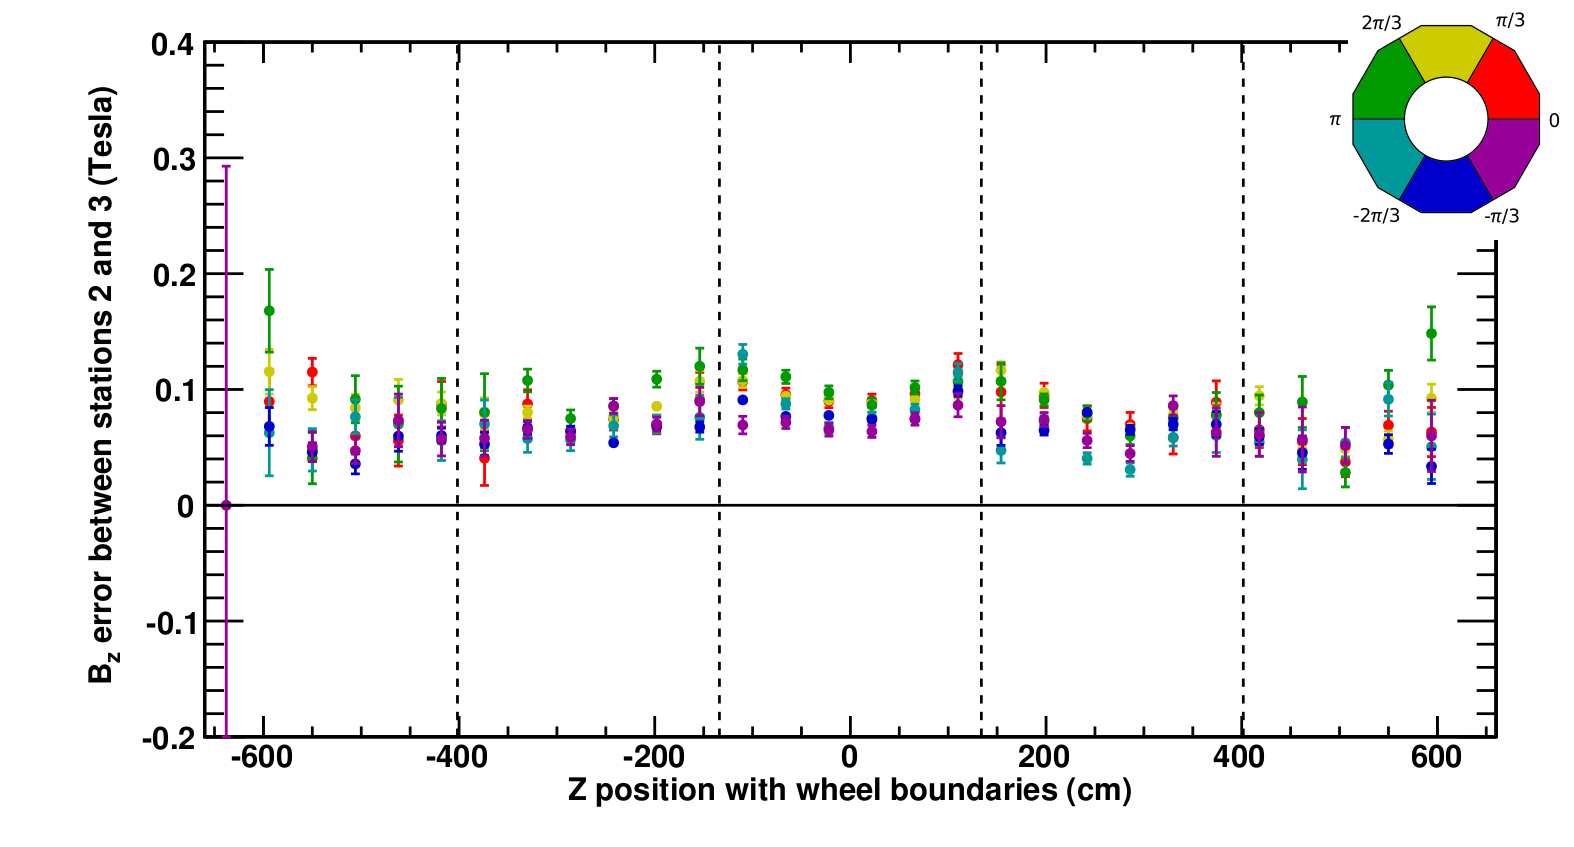
\includegraphics[width=0.95\linewidth]{berror23.png}}
\only<3>{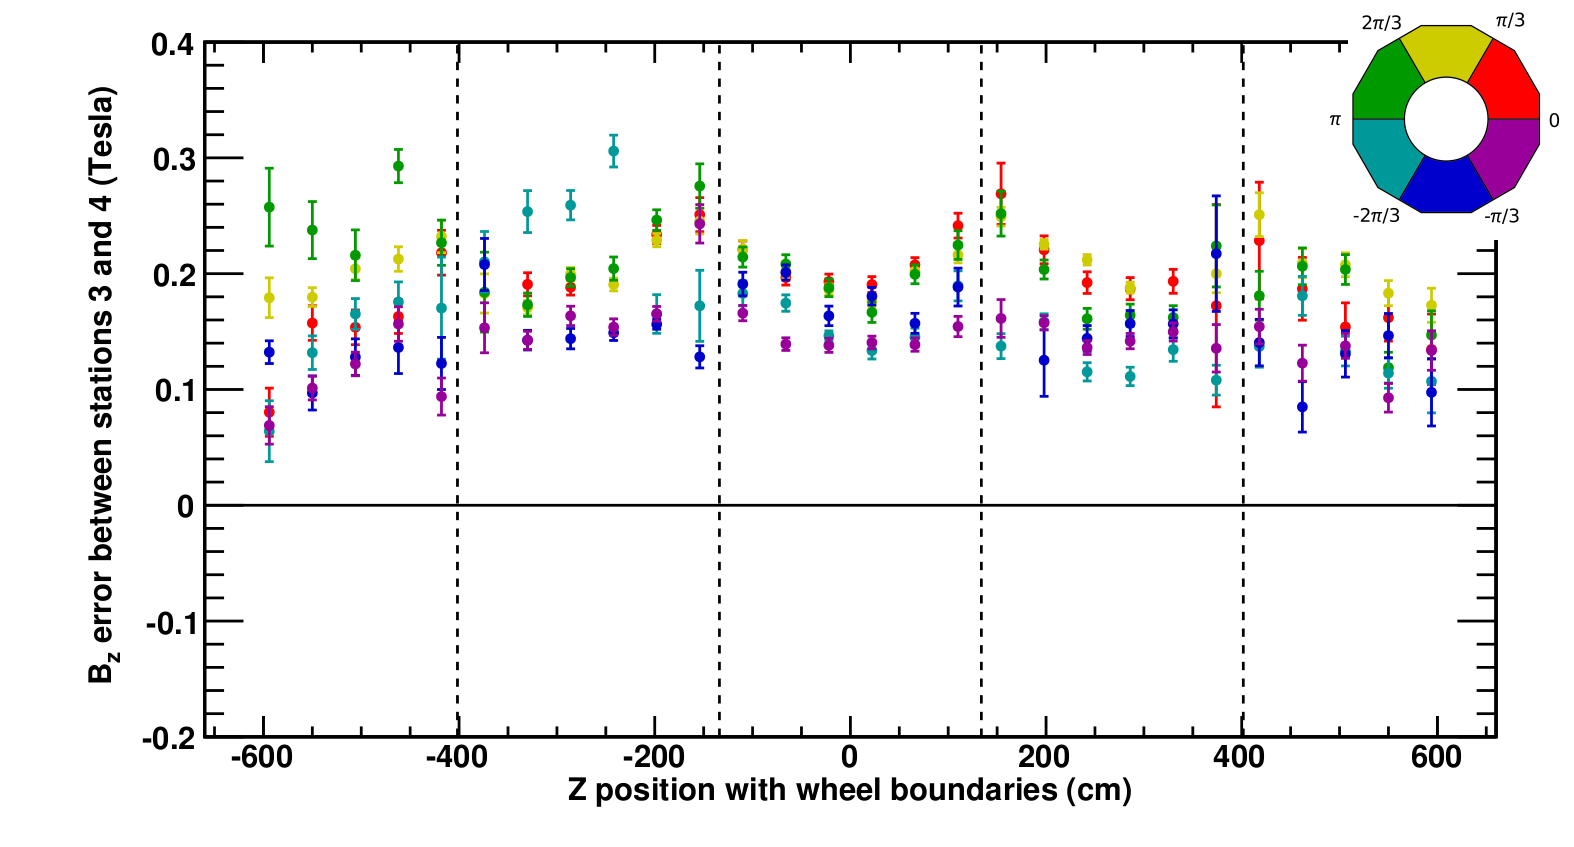
\includegraphics[width=0.95\linewidth]{berror34.png}}

\end{frame}

%% \section*{First section}
%% \begin{frame}
%% \begin{center}
%% \Huge \textcolor{blue}{First section}
%% \end{center}
%% \end{frame}

\end{document}
